%  LaTeX support: latex@mdpi.com
%  For support, please attach all files needed for compiling as well as the log file, and specify your operating system, LaTeX version, and LaTeX editor.

%=================================================================
% pandoc conditionals added to preserve backwards compatibility with previous versions of rticles

\documentclass[data,article,submit,moreauthors,pdftex]{Definitions/mdpi}


%% Some pieces required from the pandoc template
\setlist[itemize]{leftmargin=*,labelsep=5.8mm}
\setlist[enumerate]{leftmargin=*,labelsep=4.9mm}


%--------------------
% Class Options:
%--------------------

%---------
% article
%---------
% The default type of manuscript is "article", but can be replaced by:
% abstract, addendum, article, book, bookreview, briefreport, casereport, comment, commentary, communication, conferenceproceedings, correction, conferencereport, entry, expressionofconcern, extendedabstract, datadescriptor, editorial, essay, erratum, hypothesis, interestingimage, obituary, opinion, projectreport, reply, retraction, review, perspective, protocol, shortnote, studyprotocol, systematicreview, supfile, technicalnote, viewpoint, guidelines, registeredreport, tutorial
% supfile = supplementary materials

%----------
% submit
%----------
% The class option "submit" will be changed to "accept" by the Editorial Office when the paper is accepted. This will only make changes to the frontpage (e.g., the logo of the journal will get visible), the headings, and the copyright information. Also, line numbering will be removed. Journal info and pagination for accepted papers will also be assigned by the Editorial Office.

%------------------
% moreauthors
%------------------
% If there is only one author the class option oneauthor should be used. Otherwise use the class option moreauthors.

%---------
% pdftex
%---------
% The option pdftex is for use with pdfLaTeX. Remove "pdftex" for (1) compiling with LaTeX & dvi2pdf (if eps figures are used) or for (2) compiling with XeLaTeX.

%=================================================================
% MDPI internal commands - do not modify
\firstpage{1}
\makeatletter
\setcounter{page}{\@firstpage}
\makeatother
\pubvolume{1}
\issuenum{1}
\articlenumber{0}
\pubyear{2023}
\copyrightyear{2023}
%\externaleditor{Academic Editor: Firstname Lastname}
\datereceived{ }
\daterevised{ } % Comment out if no revised date
\dateaccepted{ }
\datepublished{ }
%\datecorrected{} % For corrected papers: "Corrected: XXX" date in the original paper.
%\dateretracted{} % For corrected papers: "Retracted: XXX" date in the original paper.
\hreflink{https://doi.org/} % If needed use \linebreak
%\doinum{}
%\pdfoutput=1 % Uncommented for upload to arXiv.org

%=================================================================
% Add packages and commands here. The following packages are loaded in our class file: fontenc, inputenc, calc, indentfirst, fancyhdr, graphicx, epstopdf, lastpage, ifthen, float, amsmath, amssymb, lineno, setspace, enumitem, mathpazo, booktabs, titlesec, etoolbox, tabto, xcolor, colortbl, soul, multirow, microtype, tikz, totcount, changepage, attrib, upgreek, array, tabularx, pbox, ragged2e, tocloft, marginnote, marginfix, enotez, amsthm, natbib, hyperref, cleveref, scrextend, url, geometry, newfloat, caption, draftwatermark, seqsplit
% cleveref: load \crefname definitions after \begin{document}

%=================================================================
% Please use the following mathematics environments: Theorem, Lemma, Corollary, Proposition, Characterization, Property, Problem, Example, ExamplesandDefinitions, Hypothesis, Remark, Definition, Notation, Assumption
%% For proofs, please use the proof environment (the amsthm package is loaded by the MDPI class).

%=================================================================
% Full title of the paper (Capitalized)
\Title{Estudio del gasto y duración media de los viajes de los turistas
extranjeros en distintas comunidades autónomas}

% MDPI internal command: Title for citation in the left column
\TitleCitation{Estudio del gasto y duración media de los viajes de los
turistas extranjeros en distintas comunidades autónomas}

% Author Orchid ID: enter ID or remove command
%\newcommand{\orcidauthorA}{0000-0000-0000-000X} % Add \orcidA{} behind the author's name
%\newcommand{\orcidauthorB}{0000-0000-0000-000X} % Add \orcidB{} behind the author's name


% Authors, for the paper (add full first names)
\Author{Alejandro León Líndez$^{1}$, Adrian Lizzadro Pla$^{2}$, Marta
Medina Muñiz$^{3}$}


%\longauthorlist{yes}


% MDPI internal command: Authors, for metadata in PDF
\AuthorNames{Alejandro León Líndez, Adrian Lizzadro Pla, Marta Medina
Muñiz}

% MDPI internal command: Authors, for citation in the left column

% Affiliations / Addresses (Add [1] after \address if there is only one affiliation.)
\address{%
$^{1}$ \quad Máster en Ciencia de
Datos; \href{mailto:alelin@alumni.uv.es}{\nolinkurl{alelin@alumni.uv.es}}\\
$^{2}$ \quad Máster en Ciencia de
Datos; \href{mailto:alizpla@alumni.uv.es}{\nolinkurl{alizpla@alumni.uv.es}}\\
$^{3}$ \quad Máster en Ciencia de
Datos; \href{mailto:memuiz@alumni.uv.es}{\nolinkurl{memuiz@alumni.uv.es}}\\
}

% Contact information of the corresponding author
\corres{Correspondence: Máster en Ciencia de Datos, Universitá de
Valencia.}

% Current address and/or shared authorship








% The commands \thirdnote{} till \eighthnote{} are available for further notes

% Simple summary
\simplesumm{Resumen del trabajo}

%\conference{} % An extended version of a conference paper

% Abstract (Do not insert blank lines, i.e. \\)
\abstract{Estudiar la evolución del gasto total, el gasto medio por
persona y el gasto medio diario en el periodo de 2016 a 2023 de turistas
con diversos países de residencia en distintas comunidades autónomas.
Estudio de la duración media de dichos viajes y su relación con el gasto
por persona.}


% Keywords
\keyword{keyword 1; keyword 2; keyword 3 (list three to ten pertinent
keywords specific to the article, yet reasonably common within the
subject discipline.).}

% The fields PACS, MSC, and JEL may be left empty or commented out if not applicable
%\PACS{J0101}
%\MSC{}
%\JEL{}

%%%%%%%%%%%%%%%%%%%%%%%%%%%%%%%%%%%%%%%%%%
% Only for the journal Diversity
%\LSID{\url{http://}}

%%%%%%%%%%%%%%%%%%%%%%%%%%%%%%%%%%%%%%%%%%
% Only for the journal Applied Sciences

%%%%%%%%%%%%%%%%%%%%%%%%%%%%%%%%%%%%%%%%%%

%%%%%%%%%%%%%%%%%%%%%%%%%%%%%%%%%%%%%%%%%%
% Only for the journal Data



%%%%%%%%%%%%%%%%%%%%%%%%%%%%%%%%%%%%%%%%%%
% Only for the journal Toxins


%%%%%%%%%%%%%%%%%%%%%%%%%%%%%%%%%%%%%%%%%%
% Only for the journal Encyclopedia


%%%%%%%%%%%%%%%%%%%%%%%%%%%%%%%%%%%%%%%%%%
% Only for the journal Advances in Respiratory Medicine
%\addhighlights{yes}
%\renewcommand{\addhighlights}{%

%\noindent This is an obligatory section in “Advances in Respiratory Medicine”, whose goal is to increase the discoverability and readability of the article via search engines and other scholars. Highlights should not be a copy of the abstract, but a simple text allowing the reader to quickly and simplified find out what the article is about and what can be cited from it. Each of these parts should be devoted up to 2~bullet points.\vspace{3pt}\\
%\textbf{What are the main findings?}
% \begin{itemize}[labelsep=2.5mm,topsep=-3pt]
% \item First bullet.
% \item Second bullet.
% \end{itemize}\vspace{3pt}
%\textbf{What is the implication of the main finding?}
% \begin{itemize}[labelsep=2.5mm,topsep=-3pt]
% \item First bullet.
% \item Second bullet.
% \end{itemize}
%}


%%%%%%%%%%%%%%%%%%%%%%%%%%%%%%%%%%%%%%%%%%


% tightlist command for lists without linebreak
\providecommand{\tightlist}{%
  \setlength{\itemsep}{0pt}\setlength{\parskip}{0pt}}

% From pandoc table feature
\usepackage{longtable,booktabs,array}
\usepackage{calc} % for calculating minipage widths
% Correct order of tables after \paragraph or \subparagraph
\usepackage{etoolbox}
\makeatletter
\patchcmd\longtable{\par}{\if@noskipsec\mbox{}\fi\par}{}{}
\makeatother
% Allow footnotes in longtable head/foot
\IfFileExists{footnotehyper.sty}{\usepackage{footnotehyper}}{\usepackage{footnote}}
\makesavenoteenv{longtable}



\begin{document}



%%%%%%%%%%%%%%%%%%%%%%%%%%%%%%%%%%%%%%%%%%

\section{Introducción}\label{introducciuxf3n}

El turismo es uno de los sectores claves de la economía española. España
se encuentra entre uno de los mayores destinos turísticos del mundo y
una gran parte de este proviene de extranjeros. En este trabajo, se
realiza un análisis detallado del gasto total, el gasto medio y la
duración media de los viajes realizados por turistas extranjeros en
diversas comunidades autónomas de España durante el periodo comprendido
entre los años 2016 y 2020.

La identificación de patrones de gasto y comportamiento turístico puede
aportar información valiosa por lo que se pretende responder a preguntas
como cuáles son las comunidades autónomas con mayor gasto turístico, qué
factores podrían estar relacionados con la duración media de las
estancias, y cómo ha evolucionado a lo largo del tiempo.

El periodo de estudio es especialmente interesante, ya que incluye tanto
años de relativa estabilidad económica como el inicio de la pandemia de
COVID-19, que tuvo un impacto significativo en el sector turístico
debido a la gran cantidad de restricciones impuestas, y también los años
posteriores donde estudiaremos si ha habido una recuperación a niveles
prepandémicos

\section{Carga de librerías e importación del
fichero}\label{carga-de-libreruxedas-e-importaciuxf3n-del-fichero}

Antes de comenzar, eliminamos todas las variables guardadas y cargamos
todas las librerías a emplear (readr, dplyr, tidyr,ggplot2,sf,
giscoR,ggiraph,GGally,ggridges\ldots) e importamos los datos
``Gasto\_turistas\_internacionales\_segun\_comunidad\_paisresidencia.csv''
obtenidos de la base de datos del Instituto Nacional de Estadística
(INE).

\section{Preparación de los datos}\label{preparaciuxf3n-de-los-datos}

\subsection{Tranformación a tidydata}\label{tranformaciuxf3n-a-tidydata}

Antes de comenzar con el preprocesamiento de los datos, observamos el
conjunto de datos importado en la Tabla \ref{tab:unnamed-chunk-4}.

\begin{table}[H]

\caption{\label{tab:unnamed-chunk-4}10 primeras filas de los datos importados}
\begin{adjustwidth}{-\extralength}{0cm}
             \small
\begin{tabular}[t]{cccccc}
\toprule
País de residencia & Total Nacional y CCAA & Tipo de dato & Gastos y duración media de los viajes & Periodo & Total\\
\midrule
Total & Total & Dato base & Gasto total & 2023 & 108.789,41\\
Total & Total & Dato base & Gasto total & 2022 & 87.138,19\\
Total & Total & Dato base & Gasto total & 2021 & 34.903,37\\
Total & Total & Dato base & Gasto total & 2020 & 19.786,78\\
Total & Total & Dato base & Gasto total & 2019 & 91.911,97\\
Total & Total & Dato base & Gasto total & 2018 & 89.750,75\\
Total & Total & Dato base & Gasto total & 2017 & 87.003,93\\
Total & Total & Dato base & Gasto total & 2016 & 77.415,54\\
Total & Total & Dato base & Gasto medio por persona & 2023 & 1.277\\
Total & Total & Dato base & Gasto medio por persona & 2022 & 1.216\\
\bottomrule
\end{tabular}
    \end{adjustwidth}
\end{table}

Transformamos este conjunto de datos a un conjunto tidy, donde cada
variable se encuentre en una columna y eliminamos filas que no vamos a
emplear en el estudio (tasa de variación) y columnas redudantes o que
contienen información irrelevante.De esta manera, obtenemos 4 variables
a partir de la columna Gastos y duración media de los viajes: el gasto
total, el gasto medio por persona, el gasto medio diario por persona y
la duración media de los viajes; cuyos valores son los correspondientes
a la columna Total. Por otro lado, en la columna Tipo de dato contamos
con dos valores: Dato base y Tasa de variación anual. Vamos a trabajar
únicamente con los datos base, por lo que eliminamos las filas
correspondientes a Tasa de variación anual y eliminamos la columna Tipo
de dato, que ahora aporta información redundante. Renombramos las
columnas de manera apropiada (sin espacios y con nombres representativos
de las variables). Los nombres de las variables son los siguientes:
Pais, CCAA, Periodo, Gasto\_total, Gasto\_medio\_persona,
Gasto\_medio\_diario\_persona y Duracion\_media.

\subsection{Transformación de clases}\label{transformaciuxf3n-de-clases}

Todas las variables han sido importadas como tipo carácter.
Transformamos las variables Gasto\_total, Gasto\_medio\_persona,
Gasto\_medio\_diario\_persona y Duracion\_media a numérico, donde
previamente transformamos la cadena de carácteres a una que sea
interpretable como número para poder aplicar la función as.numeric()
correctamente (eliminando el punto de miles y sustituyendo la coma
decimal por un punto decimal). Comprobamos si al realizar la
transformación se han introducido datos NA y a continuación,
transformamos a factor las variables Pais y CCAA.

Quitamos algunas filas que contienen datos que consisten en la suma
total de los datos de la columna CCA (más adelante eliminaremos también
los valores correspondientes a Total de la variable Pais). Sin embargo,
recogeremos estos valores en datasets datos\_totales y
datos\_total\_por\_residencia para hacer uso de ellos y obtener
información relevante. Cambiamos los nombres de los niveles del factor
CCAA a los siguientes: ``Andalucía'', ``Illes Balears'',``Canarias'',
``Cataluña'',``Comunitat Valenciana'', ``Comunidad de Madrid'', ``Otras
CCAA''.

\subsection{Instance engineering}\label{instance-engineering}

Vamos a trabajar con valores de las filas para obtener un dataset más
apropiado al estudio que deseamos realizar. En primer lugar, queremos
deshacernos del nivel ``Total'' en la variable Pais y transformarla en
otro llamado ``Otros'' en que en el resto de variables contenga la
información referente al resto de paises distintos de los cuáles
poseemos datos concretos.

\subsubsection{Instance engineering de
Gasto\_total}\label{instance-engineering-de-gasto_total}

Para la variable Gasto\_total, las filas correspondientes a ``Otros'' de
la variable Pais y las filas correspondientes a ``Total'' se relacionan
de la siguiente manera con \(pais\in\) \{Alemania, Francia, Italia,
Países Nórdicos, Reino Unido\}:

\[ \text{Gasto total}_{\text{Total}} = \sum_{pais}{\text{Gasto total}_{pais}}\]
Luego el gasto total de ``Otros'' es el gasto de los valores ``Total''
de Pais menos el gasto de cada uno de los otros 5 paises disponibles por
separado.

\subsubsection{Instance engineering de Gasto\_medio\_persona,
Gasto\_medio\_diario\_persona y
Duracion\_media}\label{instance-engineering-de-gasto_medio_persona-gasto_medio_diario_persona-y-duracion_media}

Como en estas variables se trata de una media, no podemos emplear el
método usado para Gasto\_total. En su lugar consideramos una media
ponderada. Si consideramos que el número de paises totales es 194
tenemos que para \(pais \in\) \{Alemania, Francia, Italia, Países
Nórdicos, Reino Unido\}:

\[
 \overline{Media\ Total} = \frac{5}{194}*\sum_{pais}{Valor\ medio}_{pais} + \frac{194-5}{194}*Valor \ Medio_{otros}
\]

De esta manera, concemos el valor de \(\overline{Media\ Total}\) y de
\({Valor\ medio}_{pais}\) y podemos calcular el valor de los valores
medios para las filas ``Otros'' de la variable Pais, otorgándoles un
mayor peso de manera proporcional al número de países considerados en
esta categoría.

\section{Resumen de los datos}\label{resumen-de-los-datos}

Una vez hemos concluido el pre-procesamiento de los datos, observamos el
resultado en la Tabla \ref{tab:unnamed-chunk-27}.

\begin{table}[H]

\caption{\label{tab:unnamed-chunk-27} 10 primeras filas del conjunto de datos procesados}
             \begin{adjustwidth}{-\extralength}{0cm}
             \small
\begin{tabular}[t]{lccccccc}
\toprule
  & Pais & CCAA & Periodo & Gasto\_total & Gasto\_medio\_persona & Gasto\_medio\_diario\_persona & Duracion\_media\\
\midrule
1 & Alemania & Andalucía & 2016 & 1121.33 & 1132 & 102 & 11.14\\
2 & Alemania & Andalucía & 2017 & 1258.89 & 1123 & 105 & 10.70\\
3 & Alemania & Andalucía & 2018 & 1256.69 & 1165 & 114 & 10.18\\
4 & Alemania & Andalucía & 2019 & 1168.38 & 1048 & 117 & 8.96\\
5 & Alemania & Andalucía & 2020 & 255.96 & 1056 & 102 & 10.34\\
6 & Alemania & Andalucía & 2021 & 464.01 & 1040 & 100 & 10.39\\
7 & Alemania & Andalucía & 2022 & 1045.65 & 1211 & 113 & 10.69\\
8 & Alemania & Andalucía & 2023 & 1314.95 & 1267 & 130 & 9.71\\
17 & Alemania & Illes Balears & 2016 & 4436.99 & 961 & 129 & 7.44\\
18 & Alemania & Illes Balears & 2017 & 4890.66 & 1013 & 133 & 7.63\\
\bottomrule
\end{tabular}
    \end{adjustwidth}
\end{table}

Vamos un resumen de los datos y de las variables disponibles. En la
Tabla \ref{tab:codebook} se ha realizado un pequeño codebook con las
variables del dataset.

\begin{table}[H]
 \caption{\label{tab:codebook} Descripción de las variables}
             \begin{adjustwidth}{-\extralength}{0cm}
             \small
             \centering
\begin{tabular}{@{}ccc@{}}
\toprule
Nombre variable & Unidad & Valores \\ \midrule
Pais & - & \begin{tabular}[c]{@{}c@{}}Alemania, Italia, Países Nórdicos, Francia, \\ Reino Unido, Otros\end{tabular} \\
CCAA & - & \begin{tabular}[c]{@{}c@{}}Andalucía, Illes Balears, Canarias, Cataluña, Comunitat Valenciana, \\ Comunidad de Madrid, Otras CCAA\end{tabular} \\
Periodo & Año & 2016-2023 \\
Gasto\_total & Millones de euros & Numérico \\
Gasto\_medio\_persona & Euros & Numérico \\
Gasto\_medio\_diario\_persona & Euros & Numérico \\
Duración\_media & Días & Numérico \\ \bottomrule
\end{tabular}


\end{adjustwidth}
\end{table}

Finalmente, antes de comenzar a visualizar datos y detectar patrones
vemos un pequeño resumen de los datos:

\begin{longtable}[]{@{}
  >{\raggedright\arraybackslash}p{(\columnwidth - 8\tabcolsep) * \real{0.0349}}
  >{\raggedright\arraybackslash}p{(\columnwidth - 8\tabcolsep) * \real{0.1977}}
  >{\raggedright\arraybackslash}p{(\columnwidth - 8\tabcolsep) * \real{0.2791}}
  >{\raggedright\arraybackslash}p{(\columnwidth - 8\tabcolsep) * \real{0.3140}}
  >{\raggedright\arraybackslash}p{(\columnwidth - 8\tabcolsep) * \real{0.1744}}@{}}
\toprule\noalign{}
\begin{minipage}[b]{\linewidth}\raggedright
\end{minipage} & \begin{minipage}[b]{\linewidth}\raggedright
Gasto total
\end{minipage} & \begin{minipage}[b]{\linewidth}\raggedright
Gasto medio por persona
\end{minipage} & \begin{minipage}[b]{\linewidth}\raggedright
Gasto medio diario/persona
\end{minipage} & \begin{minipage}[b]{\linewidth}\raggedright
Duración media
\end{minipage} \\
\midrule\noalign{}
\endhead
\bottomrule\noalign{}
\endlastfoot
& Min. : 22.28 & Min. : 383.0 & Min. : 56.0 & Min. : 3.610 \\
& 1st Qu.: 396.06 & 1st Qu.: 838.2 & 1st Qu.:107.8 & 1st Qu.: 6.060 \\
& Median : 857.80 & Median :1003.0 & Median :132.0 & Median : 7.630 \\
& Mean : 2714.09 & Mean :1005.2 & Mean :135.9 & Mean : 7.756 \\
& 3rd Qu.: 2562.09 & 3rd Qu.:1165.5 & 3rd Qu.:156.0 & 3rd Qu.: 9.198 \\
& Max. :21318.75 & Max. :1743.9 & Max. :300.8 & Max. :14.270 \\
\end{longtable}

\section{Primeras visualizaciones.}\label{primeras-visualizaciones.}

\begin{figure}[H]
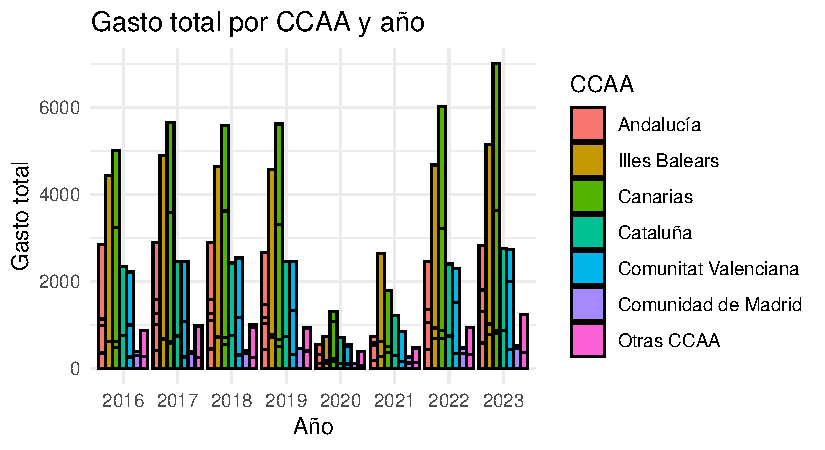
\includegraphics{ProyectoAED2024_Rmd_files/figure-latex/unnamed-chunk-22-1} \caption{Gasto total por CCAA y año.\label{fig:GastototalporCCAAyaño}}\label{fig:unnamed-chunk-22}
\end{figure}

\begin{figure}[H]
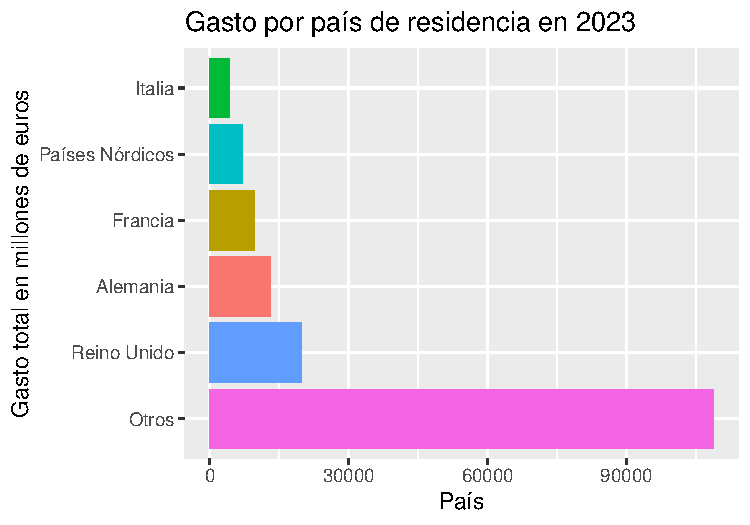
\includegraphics{ProyectoAED2024_Rmd_files/figure-latex/unnamed-chunk-23-1} \caption{Gasto total por país y CCAA .\label{fig:GastototalporpaísyCCAA}}\label{fig:unnamed-chunk-23}
\end{figure}

\begin{figure}[H]
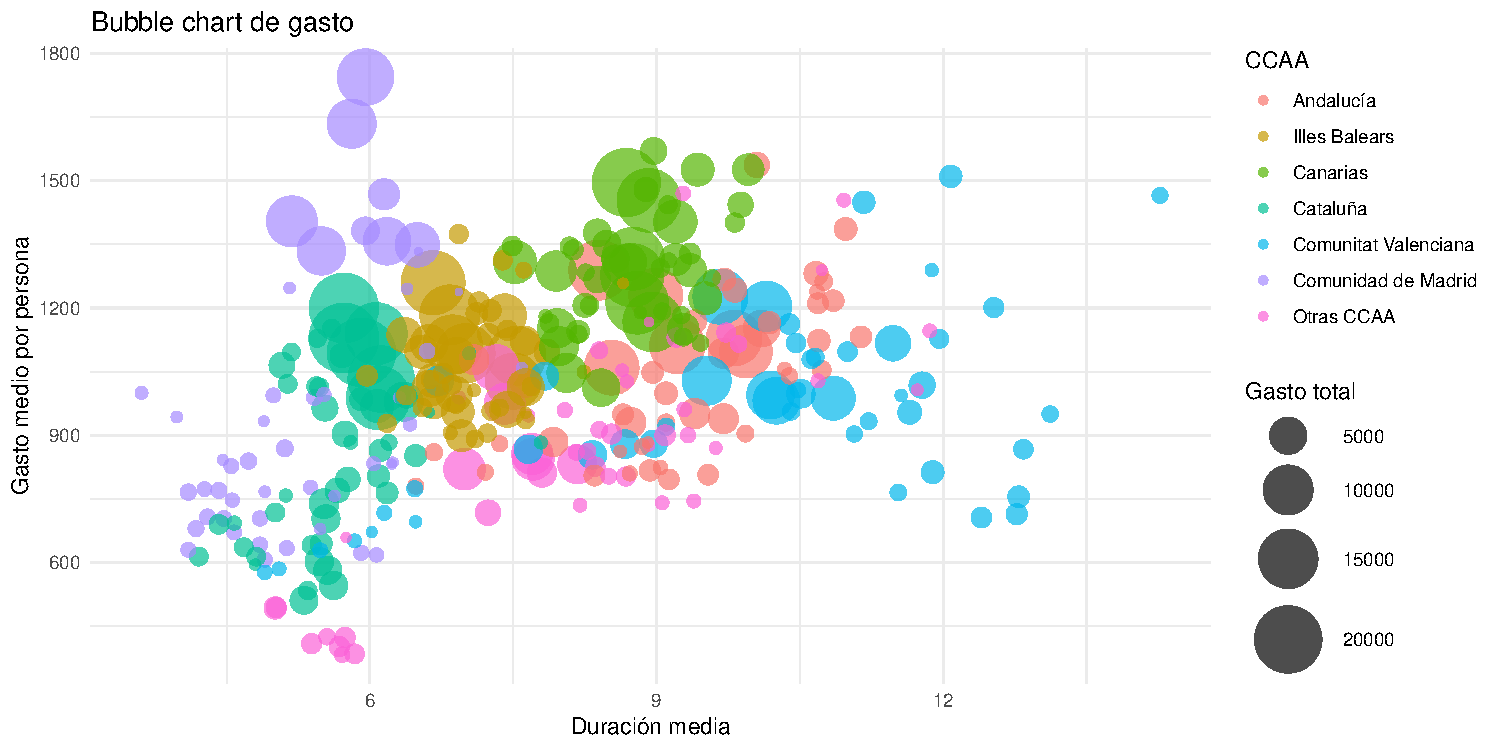
\includegraphics{ProyectoAED2024_Rmd_files/figure-latex/unnamed-chunk-24-1} \caption{Gasto medio por persona en función de duración media, CCAA y gasto total. .\label{fig:bubblegraph}}\label{fig:unnamed-chunk-24}
\end{figure}
\begin{figure}[H]
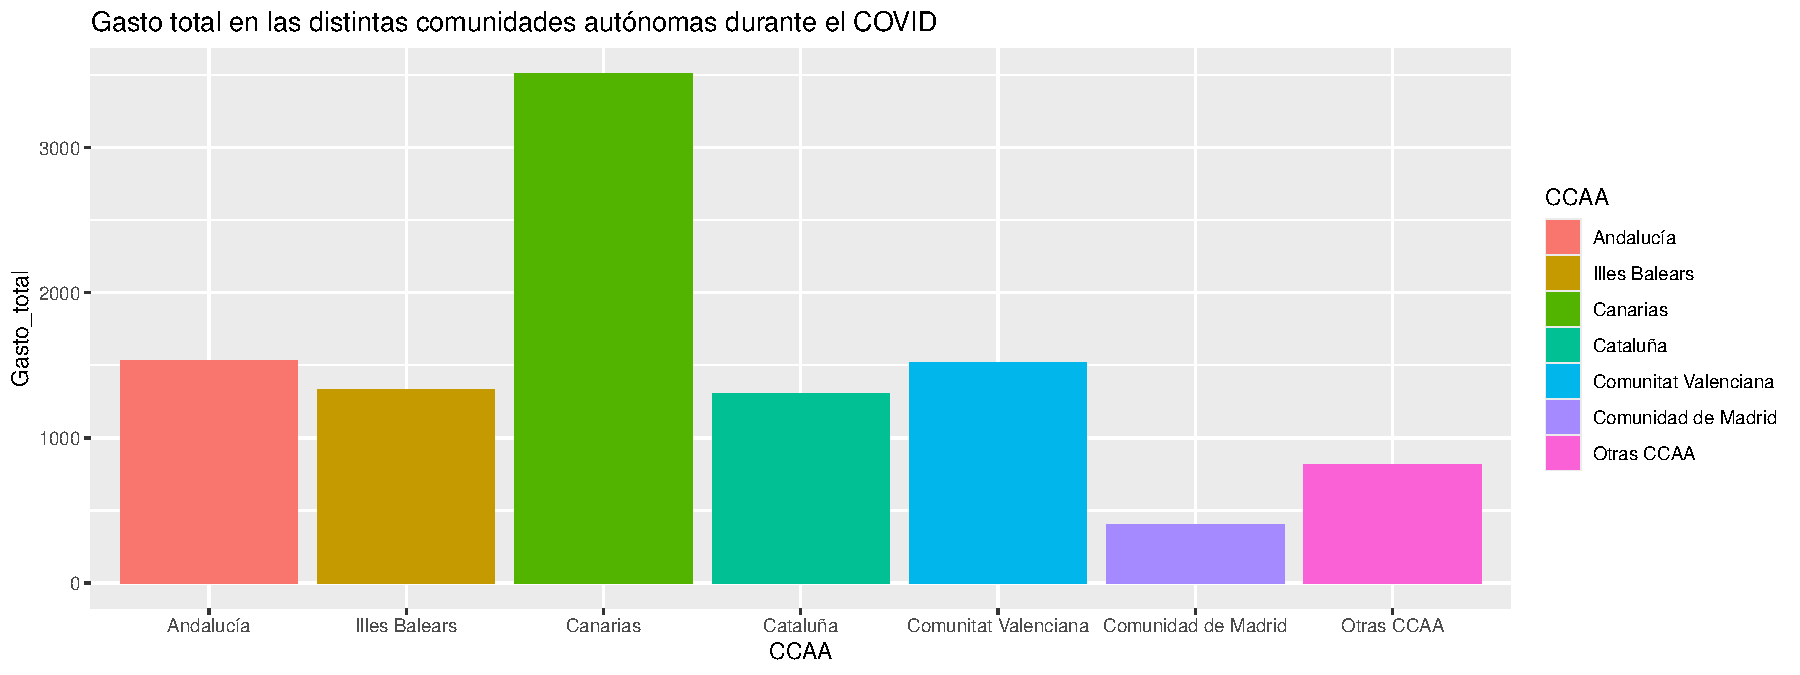
\includegraphics{ProyectoAED2024_Rmd_files/figure-latex/unnamed-chunk-25-1} \caption{Distribución del Gasto Total por País a lo largo de los Años.\label{fig:ridgelineplot}}\label{fig:unnamed-chunk-25}
\end{figure}

\begin{figure}[H]
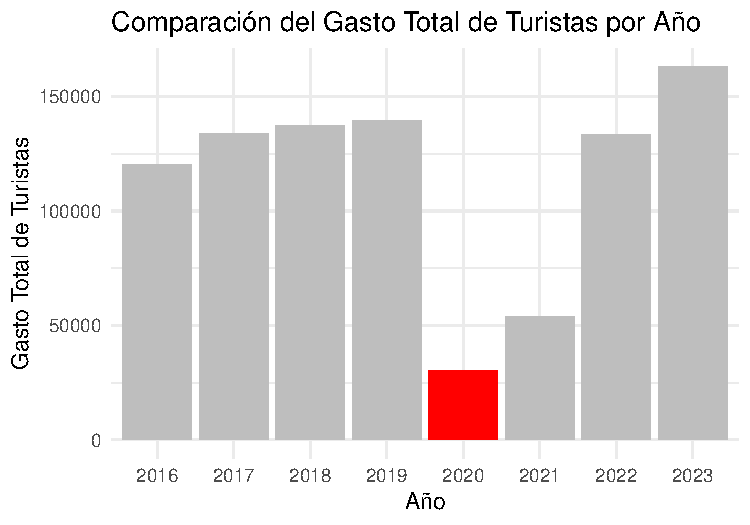
\includegraphics{ProyectoAED2024_Rmd_files/figure-latex/unnamed-chunk-26-1} \caption{Distribución de gasto medio por persona por CCAA. .\label{fig:cajas}}\label{fig:unnamed-chunk-26}
\end{figure}

\section{Efecto del covid-19}\label{efecto-del-covid-19}

Probamos a analizar el efecto del COVID en el gasto de los turistas, así
como estudiar los países que más reducieron su gasto debido a la
pandemia.

\begin{figure}[H]
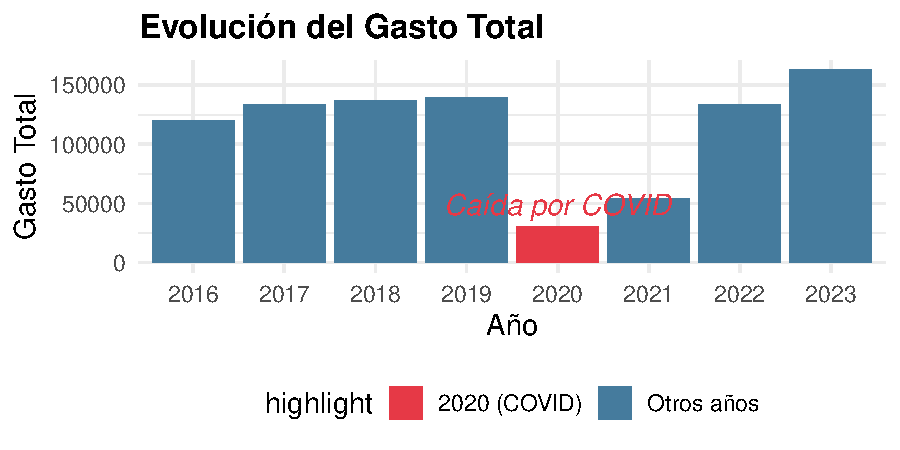
\includegraphics{ProyectoAED2024_Rmd_files/figure-latex/gasto total covid-1} \caption{Gasto total de turistas en millones de euros por año. .\label{fig:gastototalporaño}}\label{fig:gasto total covid}
\end{figure}

La media del gasto total durante el COVID es de 719.32 millones de euros
mientras que sin COVID es de 2999.06 millones de euros, una diferencia
más que notable tal y como se observa en la gráfica
\ref{fig:gastototalporaño}, con un descenso drástico en 2020 (COVID) y
una posterior recuperación. En el
gráfico\ref{fig:gastototalporpaisescovid} vemos que Reino Unido gastó
más en COVID que el resto de países, Italia el que menos.

\begin{figure}[H]
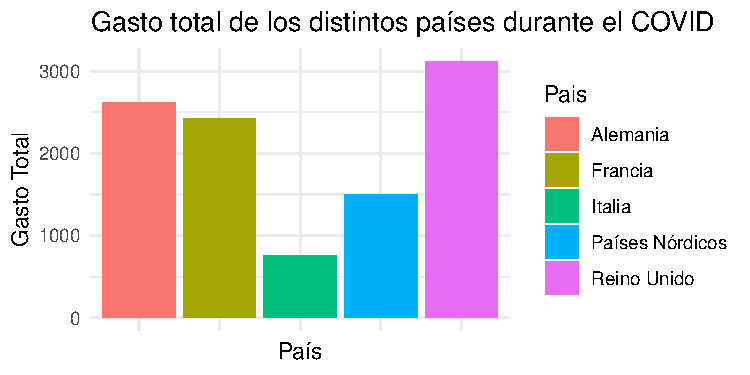
\includegraphics{ProyectoAED2024_Rmd_files/figure-latex/gasto paises covid-1} \caption{Gasto total de los distintos países durante el COVID. .\label{fig:gastototalporpaisescovid}}\label{fig:gasto paises covid}
\end{figure}

Por otro lado, podemos observar que la Comunidad Autónoma a la que más
se viajo durante el año del covid 2020 fueron las islas Canarias. Esto
puede tener diversas explicaciones. Por un lado, los primeros meses del
año, antes de las restricciones, el turismo en las islas Canarias es
mayor debido al buen tiempo incluso en los meses de invierno. Por otro
lado, el impacto del Covid en las islas puedo haber sido menor y haber
impuesto menos restricciones. Otro posible motivo es la gran dependencia
económica del turismo de las islas y una mayor disposición a atraer y
recuperar el turismo perdido lo antes posible.

\begin{figure}[H]
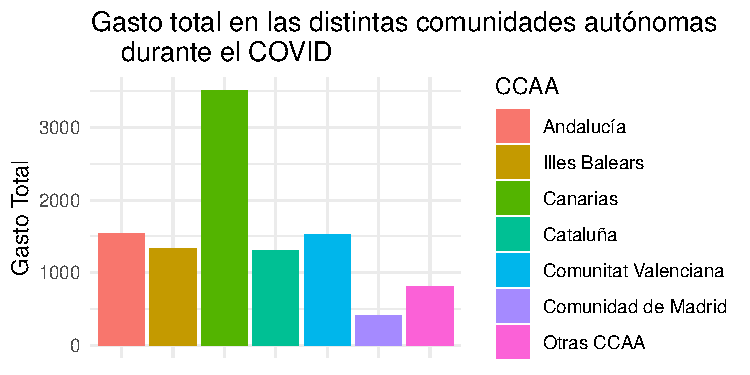
\includegraphics{ProyectoAED2024_Rmd_files/figure-latex/gasto comunidades covid-1} \caption{Gasto total en las distintas comunidades autónomas durante el COVID. .\label{fig:gastototalporCCAAcovid}}\label{fig:gasto comunidades covid}
\end{figure}

\section{Análisis bivariante de variables
cuantitativas}\label{anuxe1lisis-bivariante-de-variables-cuantitativas}

Realizamos una visualización previa para detectar relaciones entre
variables cuantitativas. En el gráfico \ref{fig:correlaciones}, se
observan 3 relaciones que podemos estudiar un poco más a fondo: el gasto
medio por persona frente al gasto medio diario, el gasto medio por
persona frente a la duración media y el gasto medio diario frente a la
duración media.

\begin{figure}[H]
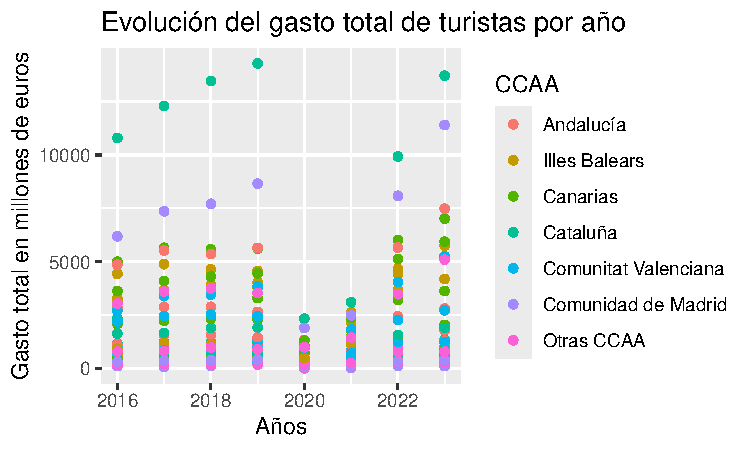
\includegraphics{ProyectoAED2024_Rmd_files/figure-latex/unnamed-chunk-28-1} \caption{Gráficos de dispersión y correlaciones entre variables cuantitativas.\label{fig:correlaciones}}\label{fig:unnamed-chunk-28}
\end{figure}

\subsection{Gasto medio por persona y duración
media}\label{gasto-medio-por-persona-y-duraciuxf3n-media}

\begin{figure}[H]
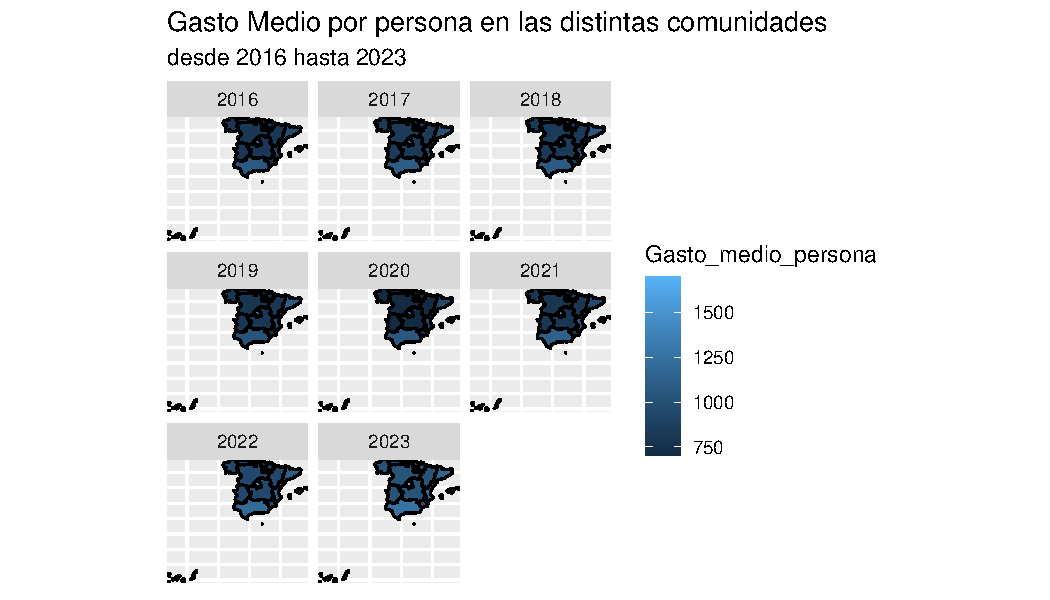
\includegraphics{ProyectoAED2024_Rmd_files/figure-latex/unnamed-chunk-29-1} \caption{Gráficos de dispersión y correlaciones entre gasto medio por persona y la duración media de los viajes .\label{fig:gastomediovsduracionmedia}}\label{fig:unnamed-chunk-29}
\end{figure}

Se observa una relación aproximadamente lineal para la mayoría de
países, donde se distinguen claramente la tendencia de duración de los
viajes en las distintas comunidades autónomas, casi siempre mayor en la
Comunitat Valenciana (salvo en Italia, probablemente por cercanía),
excepto en la categoría de otros países. Debido a que esta categoría
engloba al resto de países del mundo, es más díficil encontrar
relaciones.

\subsection{Gasto medio por persona frente al gasto medio diario por
persona}\label{gasto-medio-por-persona-frente-al-gasto-medio-diario-por-persona}

Esta parece a priori la relación más obvia entre variables.

\begin{figure}[H]
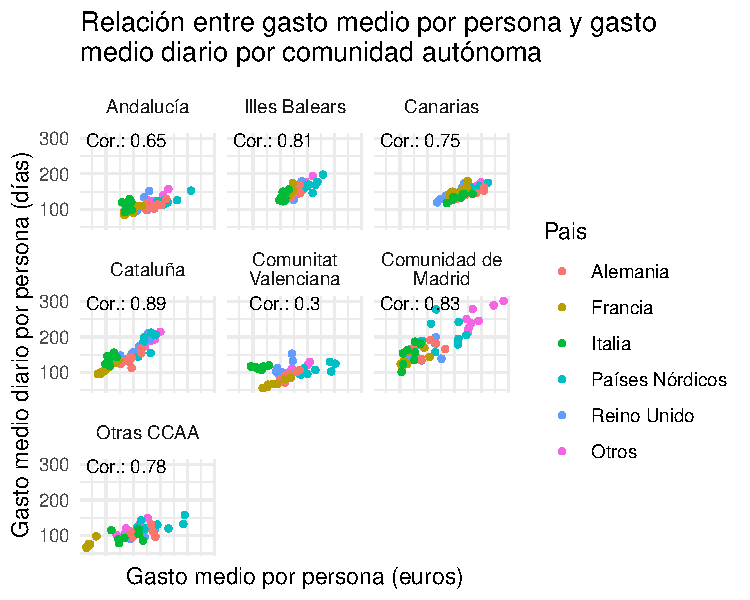
\includegraphics{ProyectoAED2024_Rmd_files/figure-latex/unnamed-chunk-30-1} \caption{Gráficos de dispersión y correlaciones entre gasto medio por persona y gasto medio diario por persona .\label{fig:gastomediovsgastomediodiario}}\label{fig:unnamed-chunk-30}
\end{figure}

En la Comunitat Valenciana es donde hay una peor correlación, esto puede
estar relacionado con que es también el destino de mayor duración de los
viajes, lo que puede provocar un menor gasto medio diario.

\begin{figure}[H]
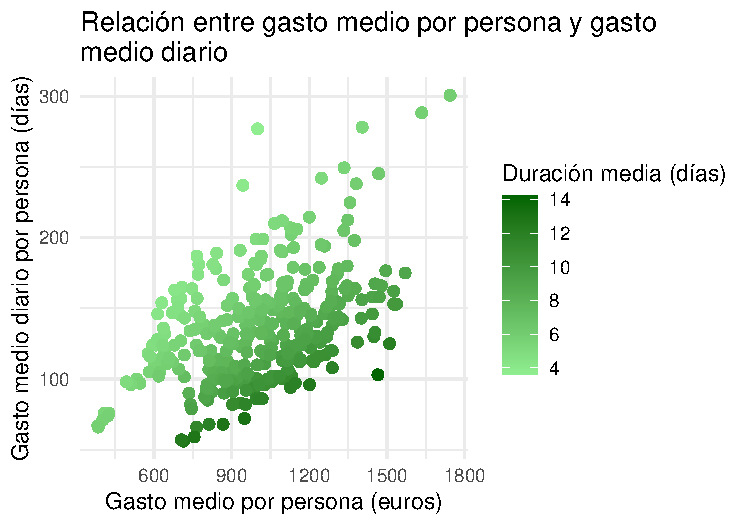
\includegraphics{ProyectoAED2024_Rmd_files/figure-latex/unnamed-chunk-31-1} \caption{Gráfico de dispersión entre gasto medio por persona y gasto medio diario .\label{fig:gastomediovsgastomediodiarioconduracion}}\label{fig:unnamed-chunk-31}
\end{figure}

En el gráfico \ref{fig:gastomediovsgastomediodiarioconduracion} se puede
ver que generalmente a mayor gasto medio por persona también se produce
un mayor gasto medio diario. Sin embargo, observamos que aparentemente
un aumento de la duración de los viajes provoca una disminución del
gasto medio diario. Vamos a visualizar esto más claramente a
continuación.

\subsection{Gasto medio diario y duracion
media}\label{gasto-medio-diario-y-duracion-media}

\begin{figure}[H]
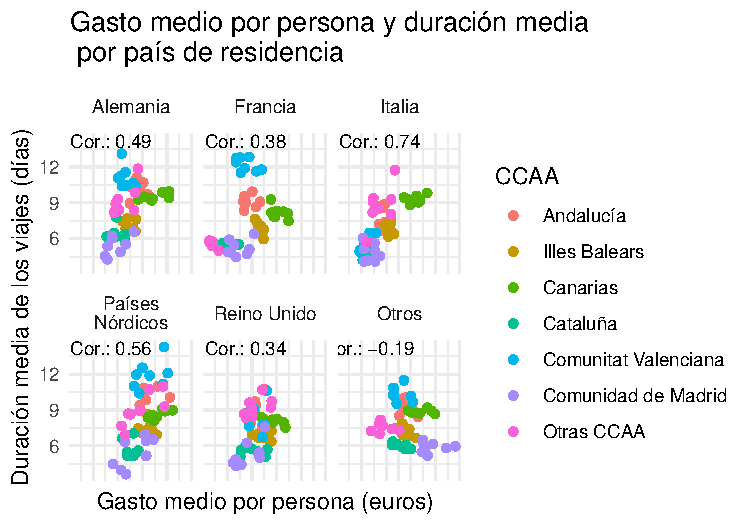
\includegraphics{ProyectoAED2024_Rmd_files/figure-latex/unnamed-chunk-32-1} \caption{Gráfico de dispersión entre gasto medio diario por persona y duración media de los viajes .\label{fig:gastomediodiariovsduracionmedia}}\label{fig:unnamed-chunk-32}
\end{figure}

Ahora podemos observar en el Gráfico
\ref{fig:gastomediodiariovsduracionmedia} de manera clara que a mayor
duración de los viajes se produce un menor gasto medio por persona.

%%%%%%%%%%%%%%%%%%%%%%%%%%%%%%%%%%%%%%%%%%

\vspace{6pt}

%%%%%%%%%%%%%%%%%%%%%%%%%%%%%%%%%%%%%%%%%%
%% optional

% Only for the journal Methods and Protocols:
% If you wish to submit a video article, please do so with any other supplementary material.
% \supplementary{The following supporting information can be downloaded at: \linksupplementary{s1}, Figure S1: title; Table S1: title; Video S1: title. A supporting video article is available at doi: link.}

%%%%%%%%%%%%%%%%%%%%%%%%%%%%%%%%%%%%%%%%%%







%%%%%%%%%%%%%%%%%%%%%%%%%%%%%%%%%%%%%%%%%%
%% Optional

%% Only for journal Encyclopedia


%%%%%%%%%%%%%%%%%%%%%%%%%%%%%%%%%%%%%%%%%%
%% Optional
\input{"appendix.tex"}
%%%%%%%%%%%%%%%%%%%%%%%%%%%%%%%%%%%%%%%%%%
\begin{adjustwidth}{-\extralength}{0cm}

%\printendnotes[custom] % Un-comment to print a list of endnotes


\reftitle{References}
\bibliography{mybibfile.bib}

% If authors have biography, please use the format below
%\section*{Short Biography of Authors}
%\bio
%{\raisebox{-0.35cm}{\includegraphics[width=3.5cm,height=5.3cm,clip,keepaspectratio]{Definitions/author1.pdf}}}
%{\textbf{Firstname Lastname} Biography of first author}
%
%\bio
%{\raisebox{-0.35cm}{\includegraphics[width=3.5cm,height=5.3cm,clip,keepaspectratio]{Definitions/author2.jpg}}}
%{\textbf{Firstname Lastname} Biography of second author}

%%%%%%%%%%%%%%%%%%%%%%%%%%%%%%%%%%%%%%%%%%
%% for journal Sci
%\reviewreports{\\
%Reviewer 1 comments and authors’ response\\
%Reviewer 2 comments and authors’ response\\
%Reviewer 3 comments and authors’ response
%}
%%%%%%%%%%%%%%%%%%%%%%%%%%%%%%%%%%%%%%%%%%
\PublishersNote{}
\end{adjustwidth}


\end{document}
